First, we will go through the main challenges for solving \eqref{eq:FPE-0--dynamic-fp} in high dimensions. These challenges and their solutions will naturally lead us to an algorithm for solving high-dimensional FPEs. Lastly, we will discuss various nuances associated with this algorithm.

\subsection{Failure of the physics-informed way}
 Since we used deep learning to find zeros of the Fokker-Planck operator in the prequel \cite{mandal2023learning}, the most natural question becomes does an analogous algorithm work for time-dependent FPEs? For an overview of learning solutions to PDEs in a \textit{physics-informed} fashion see section 5 of \cite{mandal2023learning} or \cite{raissi2019physics}, \cite{blechschmidt2021three}, \cite{sirignano2018dgm}. 
As noted in section 5 of \cite{mandal2023learning} the first step to learning the solution to a PDE is to convert it into an optimization problem. For notational convenience let us first define the function space $\mathcal F$ as follows,
\begin{align}
\mathcal F\stackrel{\rm def}{=}\{&f:[0, T]\times\mathbb R^d\to[0, +\infty):\int_{\mathbb R^d}f(t, \mathbf x)\,d\mathbf x=1\;\forall\; t\in[0, T]\}\label{eq:def-fn-space--dynamic-fp}
\end{align}

Proceeding parallely to section 5 of \cite{mandal2023learning} or \cite{sirignano2018dgm} we might be tempted to solve the following optimization problem,
\begin{align}
    \underset{f\in\mathcal F }{\rm arg\,inf}\;\mathcal J(f)\stackrel{\rm def}{=}\underset{f\in\mathcal F }{\rm arg\,inf}\left[\frac{1}{MN}\sum_{i=1}^M\sum_{j=1}^N\left(\frac{\partial f}{\partial t}(t_i, \mathbf x_j)-\mathcal Lf(t_i, \mathbf x_j)\right)^2+ \frac{1}{N}\sum_{j=1}^N(f(0, \mathbf x_j)-p_0(\mathbf x_j))^2\right]\label{eq:dynamic-opt--dynamic-fp}
\end{align}
where $\{\mathbf x_j\}_{j=1}^N$ is a uniform sample from our compact  domain of interest $\Omega_I$ (see section 6.1 in \cite{mandal2023learning}) and $\{t_i\}_{i=1}^M$ is a sample from $[0,T]$.
But it turns out problem \eqref{eq:dynamic-opt--dynamic-fp} is not a \textit{well-behaved} problem. The following proposition explains why this is the case.
\begin{prop}
    Suppose \eqref{eq:FPE-0--dynamic-fp} has a unique, strong solution $p$ and 
    \begin{align}
        \mathcal Lf = 0\label{eq:SFPE--dynamic-fp}
    \end{align}
    also has a unique, strong, probability solution $p_\infty$. 
    Then there exists a sequence of functions $f_k\in\mathcal F$ independent of the samples $\{\mathbf x_j\}_{j=1}^N, \,\{t_i\}_{i=1}^M$ such that \begin{align}
        \lim_{k\to+\infty}\mathcal J(f_k) = 0
\end{align}
    but
    \begin{align}
        \lim_{k\to+\infty}f_k\neq p
    \end{align}\label{prop:failure--dynamic-fp}
\end{prop}
\begin{proof}
WLOG assume that $\{t_i\}_{i=1}^M$ is ordered and $0=t_1<t_2<\cdots<t_M$. Since we have included $t_1=0$ in our sample, while considering $\frac{\partial}{\partial t}$ at $t=t_1=0$ we'll only consider the right derivative.
For $k\in\mathbb N$ define the sequence,
\begin{align}
    f_{k}(t, \mathbf x) =\begin{cases}
    &p(t,\mathbf x),\;\;t\le\frac{1}{k}\\
    &\phi_k(t)\,p(t, \mathbf x) + (1-\phi_{k}(t))\,p_\infty(\mathbf x),\;\; t>\frac{1}{k}
    \end{cases}
\end{align}
where,
\begin{align}
    \phi_{k}(t) = e^{1-kt}
\end{align}
Since $p,p_\infty$ are probability densities, it is easy to see that  $f_k\in\mathcal F,\;\;\forall\, k\in\mathbb N$.
The second term or the initial condition term in $\mathcal J(f_k)$ vanishes since $f_k(0,\mathbf x)=p(0,\mathbf x)=p_0(\mathbf x)$. Moreover since $p$ is a zero of $\frac{\partial}{\partial t}-\mathcal{L}$, 
\begin{align}
    \sum_{j=1}^N\left(\frac{\partial f_k}{\partial t}(t_1, \mathbf x_j)-\mathcal Lf_k(t_1, \mathbf x_j)\right)^2 =0
\end{align}
where as noted before we have only considered the right time-derivative at  $t=t_1=0$. Now pick $K>0:\frac{1}{K}<t_2$. For $k>K$, using the fact that $p, p_\infty$ are both zeros of $\frac{\partial}{\partial t}-\mathcal{L}$ we see that,
\begin{align}
    \mathcal J(f_{k})=&\frac{1}{MN}\sum_{i=2}^M\sum_{j=1}^N\left(\frac{d \phi_k}{d t}(t_i)(p_\infty(\mathbf x_j)-p(t_i, \mathbf x_j))\right)^2
\end{align}
Due to continuity of $p,p_\infty$ and compactness of $\Omega_I$ there exists $B\ge0:$ 
    \begin{align}
        \sup\left\{p(t, \mathbf x)^2, p_\infty(\mathbf x)^2 :t\in[0, T],\;\mathbf x\in\Omega_I\right\}= B
    \end{align}
which implies $\;\forall\;k>K$,
\begin{align}
    \mathcal{J}(f_k)\le&\frac{2B}{MN}\sum_{i=2}^M\sum_{j=1}^N\left(\frac{d \phi_k}{d t}(t_i)\right)^2=\frac{2Be^2k^2}{MN}\sum_{i=2}^M\sum_{j=1}^Ne^{-2kt_i}
<{2Be^2k^2}e^{-2kt_2}
\end{align}
Since $t_2>0$ we have
\begin{align}
    \lim_{k\to+\infty}\mathcal J(f_k)=0
\end{align}
But clearly the pointwise limit of $f_k$ is given by
\begin{align}
    f(t, \mathbf x) =\begin{cases}
    &p_0(\mathbf x),\;\;t=0\\
    &p_\infty(\mathbf x),\;\; t>0
    \end{cases}\label{eq:limit-min-seq--dynamic-fp}
\end{align}
\end{proof}
The proof assumes very little about the operator $\mathcal L$ and hence can be extended to other partial differential equations of parabolic type. Only assumptions required to prove proposition~\ref{prop:failure--dynamic-fp} are the existence of strong, unique probability solutions which are true for all of our example problems, see appendix 9.1 in \cite{mandal2023learning} and appendix~\ref{ssec-unique--dynamic-fp} in this paper. Since we only have finite computational resources it is sensible to investigate loss functions with finite sample-sizes and note that the proof of proposition~\ref{prop:failure--dynamic-fp} works for any choice of samples $\{t_i\}_{i=1}^M,\,\{\mathbf x_j\}_{j=1}^N$ with arbitrary but finite sample-sizes. Note that the pathological sequence we constructed is independent of the samples $\{t_i\}_{i=1}^M,\,\{\mathbf x_j\}_{j=1}^N$ which is an important component of the failure of the physics-informed way. In the case of stationary Fokker-Planck equations we can also construct pathological functions that make the physics-informed loss (defined in section~6.3 of \cite{mandal2023learning}) vanish without converging to a solution by simply interpolating a solution at the sample points with non-solutions at unsampled points. But the physics-informed method still produces correct solutions in the stationary case since these pathological functions are sample-dependent and as the sample-size increases, they resemble a solution more and more closely. From the perspective of training a neural network to optimize problem~\ref{eq:dynamic-opt--dynamic-fp} the main difficulty is revealed by the limit of the minimizing sequence given in \eqref{eq:limit-min-seq--dynamic-fp}. The network can behave like the initial condition for a short amount of time and then mimic $p_\infty$ for all subsequent times losing all variation in time. Moreover, one can construct many such sequences with pathological behaviors, not to mention restricting neural networks to $\mathcal{F}$ and have them be expressive is another challenge since normalization is an extremely difficult condition to implement in high dimensions, see the discussion in sections 2 and 6.4 of \cite{mandal2023learning}. Apart from these difficulties, for other explorations of failure modes of physics-informed neural networks see \cite{krishnapriyan2021characterizing}, \cite{basir2022investigating}.
\label{ssec-failure--dynamic-fp}

\subsection{The Feynman-Kac formula}
Due to the ineffectiveness of the physics informed method, we turn to another very useful paradigm for solving high dimensional PDEs. The Feynman-Kac formula \cite{pham2015feynman} has been used very successfully in recent years to solve high-dimensional PDEs \cite{hutzenthaler2021multilevel}. They have also been used alongside deep-learning to create algorithms for semilinear parabolic PDEs \cite{han2018solving}. Moreover, while verifying algorithms for very high dimensional PDEs one often relies on the Feynman-Kac formula to get a reference solution, see for example the examples given in sections 4, 5 of \cite{sirignano2018dgm}. The pointwise nature of the Feynman-Kac formula makes it very attractive for high-dimensional problems, since it waives the requirement for a mesh. Below we briefly discuss a few versions of the formula and the challenges associated with using it for \eqref{eq:FPE-0--dynamic-fp}.

The following version of the formula appears in \cite{oksendal2003stochastic} and it is one of the most well-known versions.
\begin{thm}[Feynman-Kac]
Suppose $f\in C^2_0(\mathbb R^d)$ and $q\in C(\mathbb R^d)$. If $q$ is bounded below then
\begin{align}
    v(t, \mathbf x) = \mathbb E\left[\left.\exp\left(-\int_0^t q(\bar X_s)\,ds\right)f(\bar X_t)\right\vert \bar X_0=\mathbf x\right]\label{eq:FK-sol--dynamic-fp}
\end{align}
is the unique solution of
\begin{equation}
\begin{aligned}
    &\frac{\partial u}{\partial t}= Au - qu\\
    & u(0, \mathbf x)=f(\mathbf x)
\end{aligned}\label{eq:FK--dynamic-fp}
\end{equation}
that's bounded on $K\times\mathbb R^d$ for every compact $K\subset[0,+\infty)$, where $\bar X_t$ is a time-homogeneous Itô process satisfying 
\begin{align}
    d\bar X_t = \bar\mu(\bar X_t)\, dt + \bar\sigma(\bar X_t)\,dW_t\label{eq:ito-time-homo--dynamic-fp}
\end{align}
with
\begin{align}
    |\bar\mu(\mathbf x)-\bar\mu(\mathbf y)| + |\bar\sigma(\mathbf x)-\bar\sigma(\mathbf y)|\le C|\mathbf x -\mathbf y|,\;\forall\,\mathbf x, \mathbf y\in\mathbb R^d\label{eq:ito-lipschitz--dynamic-fp}
\end{align}

where $C$ is a positive constant and $A$ is the infinitesimal generator of $\bar X_t$ given by 
\begin{align}
    Af = \bar\mu\cdot\nabla f + \frac{1}{2}{\rm tr}(\bar\sigma\bar\sigma^\top\odot\nabla^2f)\label{eq:ito-gen--dynamic-fp}
\end{align}
\label{thm:FK-Oksendal--dynamic-fp}\end{thm}

Note the three requirements for theorem~\ref{thm:FK-Oksendal--dynamic-fp} are global Lipschitzness of $\bar\mu$ and $\bar\sigma$, vanishing of the initial condition $f$ at infinity and the lower-boundedness of $q$. Lipschitzness of drift and diffusion coefficient ensures that SDE~\eqref{eq:ito-time-homo--dynamic-fp} has a unique, non-exploding, strong solution \cite{ikeda2014stochastic}. Vanishing of the initial condition $f$ and lower-boundedness of $q$ guarantee that the expectation in \eqref{eq:FK-sol--dynamic-fp} is bounded.

If we try to apply formula \eqref{eq:FK-sol--dynamic-fp} directly to the Fokker-Planck equation \eqref{eq:FPE-1--dynamic-fp}, we have to identify the following quantities,

\begin{equation}
\begin{aligned}
    &\bar\mu = -\mu\\
    &\bar\sigma =\sigma\\
    & q = -\nabla\cdot\mu
\end{aligned}
\end{equation}

In our examples none of the three requirements for theorem~\ref{thm:FK-Oksendal--dynamic-fp} are always satisfied. Concretely, the 2D ring system \eqref{eq:ring2D--dynamic-fp} satisfies none of the requirements. Lipschitzness of the drift is too restrictive a condition to model real world phenomena and therefore attempts have been made to relax this condition. In \cite{yamada1971uniqueness} the Lipschitz condition is replaced with Hölder condition for 1D SDEs, furthermore in \cite{fu2010stochastic}, \cite{li2011strong} sufficient conditions for existence of pathwise unique solutions of 1D SDEs have been discussed. \cite{xi2019jump} discusses the more general case when the SDEs are multi-dimensional with non-Lipschitz drifts and gives us an identical Feynman-Kac formula for \eqref{eq:FK--dynamic-fp} under the condition that \eqref{eq:ito-time-homo--dynamic-fp} has a unique, weak solution. For the sake of completeness, below we provide a special case of the more general result proved in theorem~7.5 of \cite{xi2019jump}.

\begin{thm}[Feyman-Kac with non-Lipschitz drift] Assume the following.
\begin{enumerate}
    \item \eqref{eq:ito-time-homo--dynamic-fp} has a unique weak solution.
    \item $v(\cdot,\cdot):[0, T]\times\mathbb R^d\to\mathbb R$ lies in $C^{1,2}([0, T)\times\mathbb R^d)\cap C_b([0, T]\times\mathbb R^d)$ and satisfies the Cauchy problem \eqref{eq:FK--dynamic-fp}.
    \item $f$ is uniformly bounded.
\end{enumerate}
Then $v$ is given by the formula \eqref{eq:FK-sol--dynamic-fp}.
\end{thm}







The requirement that $q$ be lower-bounded can be easily arranged while simultaneously simplifying \eqref{eq:FK-sol--dynamic-fp} by looking at an auxiliary equation. To derive this auxiliary equation we can write, 
\begin{align}
    p(t, \mathbf x) = h(t, \mathbf x)p_\infty(\mathbf x)
\end{align}
where $p_\infty$ is a nonzero zero of the operator $\mathcal L$. It is then easy to see that $h$ satisfies the equation, 
\begin{equation}
\begin{aligned}
    &h(t, \mathbf x) = (\sigma^2\nabla\log p_\infty - \mu)\cdot \nabla h + \frac{\sigma^2}{2}\Delta h,\qquad \mathbf x\in \mathbb R^d, t\in(0, T]\\
    &h(0, \mathbf x) = \frac{p_0(\mathbf x)}{p_\infty(\mathbf x)},\qquad \mathbf x\in \mathbb R^d
\end{aligned}\label{eq:h--dynamic-fp}
\end{equation}
Note that $\mathcal L$, being a linear operator, can have infinitely many distinct zeros and each such $p_\infty$ will give rise to a different PDE for $h$. If we can compute $p_\infty$ then we can compute $p$ by computing $h$. In \cite{mandal2023learning} we provide a deep learning method to compute positive zeros of $\mathcal L$ and thus for our purposes it suffices to compute $h$. To compute $h$ with the Feynman-Kac formula we identify the following quantities, 

\begin{equation}
\begin{aligned}
    &\bar\mu = (\sigma^2\nabla\log p_\infty - \mu)\\
    &\bar\sigma =\sigma\\
    & q = 0
\end{aligned}
\end{equation}

In this construction $q$ has automatically become lower-bounded. Moreover, the formula \eqref{eq:FK--dynamic-fp} simplifies to 
\begin{align}
    h(t, \mathbf x) = \mathbb E\left[\left.\frac{p_0(\bar X_t)}{p_\infty(\bar X_t)}\right\vert \bar X_0=\mathbf x\right]\label{eq:h-E--dynamic-fp}
\end{align}
where $\bar X_t$ satisfies, 
\begin{align}
    d\bar X_t = (\sigma^2\nabla\log p_\infty-\mu)\,dt + \sigma\,dW_t\label{eq:h-SDE--dynamic-fp}
\end{align}
Finally, $p(t,\mathbf x)$ can be computed with the formula, 
\begin{align}
    p(t, \mathbf x) = \mathbb E\left[\left.\frac{p_0(X_t)}{p_\infty(X_t)}\right\vert X_0=\mathbf x\right]p_\infty(\mathbf x)\label{eq:p-E--dynamic-fp}
\end{align}

Note that even if the computed $p_\infty$ is unnormalized since we both multiply and divide by $p_\infty$ in \eqref{eq:p-E--dynamic-fp}, the normalization constant cancels out. Also, since $\bar\mu$ depends on $p_\infty$ through $\nabla\log p_\infty$, the normalization constant for $p_\infty$ is again eliminated and $X_t$ appearing in \eqref{eq:p-E--dynamic-fp} is independent of the normalization constant. Therefore, we can recover the correct $p$ with \eqref{eq:p-E--dynamic-fp} for any nonzero zero of $\mathcal L$ which can be computed following the recipe laid out in \cite{mandal2023learning}. For the sake of convenience, we will refer to equations \eqref{eq:h--dynamic-fp} and \eqref{eq:h-SDE--dynamic-fp}  as the \textit{h-equation} and the \textit{h-SDE} respectively.

We have only dealt with two of the three requirements of theorem~\ref{thm:FK-Oksendal--dynamic-fp} so far by appealing to the more general version of the Feynamn-Kac formula \cite{xi2019jump} and transforming the original FPE. The remaining requirement that the initial condition vanishes at infinity translates to $\frac{p_0}{p_\infty}$ vanishing at infinity. Even though we do not impose this restriction in our examples, in section~\ref{ssec-limit--dynamic-fp} we see that this condition is immaterial to our situation since we restrict the trajectories of the h-SDE \eqref{eq:h-SDE--dynamic-fp} to a finite domain and the expectation in \eqref{eq:p-E--dynamic-fp} is therefore bounded. 



\label{ssec-Feynman-Kac--dynamic-fp}

\subsection{The algorithm}
In this section we outline the algorithm for learning zeros of FPOs. But before that we go through the primary challenges and ways to mitigate them.

\subsection{Unboundedness of the problem domain}\label{ssec-unbounded-domain--steady-fp} We can try the same procedure as outlined in section~\ref{sec-learning--steady-fp} to find a non-trivial zero of $\mathcal L$. But computationally we can only deal with a bounded domain. Hence we focus on a compact domain which contains most of the mass of the solution to \eqref{eq:SFPE-0--steady-fp}. We refer to this domain as the \textit{domain of interest} $\Omega_I$ in the following discussion. \textcolor{magenta}{We note that the support of non-trivial zeros of $\mathcal L$ will usually be unbounded and of course we do not know the domain that may contain most of the mass. Thus the choice of $\Omega_I$ needs to be informed by some a priori knowledge of the solution, which in the examples we discuss is related to some attracting set of the deterministic system associated to the drift term $\mu$, i.e., the first term in~\eqref{eq-sde--steady-fp}. We do not need a precise knowledge of such an attracting set. But the smaller the domain $\Omega_I$, the more efficient will be the proposed method which requires uniform samples from $\Omega_I$.}
%{We note two points about the choice of $\Omega_I$: (i) The support of non-trivial zeros of $\mathcal L$ will usually be unbounded}


\subsection{Existence of the trivial solution}\label{ssec-exist-0--steady-fp} \textcolor{magenta}{Since $\mathcal L$ is a linear operator, zero is a trivial solution: $\mathcal L 0 = 0$. We also note that if $\nabla \cdot \mu \not\equiv 0$, then no other constant function (other than zero) is a zero of $\mathcal L$.} Since we want to find a non-trivial zero of $\mathcal L$, we would like avoid the learning the zero function during the training of the network. To deal with this problem \cite{zhai2022deep} added a regularization term that used approximate solutions of \eqref{eq:SFPE-0--steady-fp} found using Monte-Carlo. Here we propose a method that does not require a priori knowing an approximate solution. Consider the operator $\mathcal L_{\rm log}$ instead.
\begin{align}
    \mathcal L_{\rm log}f \stackrel{\rm def}{=} e^{-f}\mathcal L e^f\label{eq:def-log-FPO--steady-fp}
\end{align}
\textcolor{magenta}{Note that if $f$ is a zero of $\mathcal L_{\rm log}$, then $p = e^f$ is a zero of $\mathcal{L}$. Further, if $f$ is bounded below on some domain within $\Omega_I$, then $p$ is a non-trivial zero of $\mathcal{L}$.} Thus we can look for a zero of $\mathcal L_{\rm log}$ to find a non-trivial zero of $\mathcal L$. Recalling \eqref{eq:log-factor-V--steady-fp} we see that,
\begin{align}
    \mathcal L_{\rm log}f=
    -\nabla\cdot \mu - \mu \cdot \nabla f + D\left(\|\nabla f\|_2^2 + \Delta f\right)\label{eq:log-FPO--steady-fp}
\end{align}
We again note that when $\nabla\cdot\mu\not\equiv0$, then any constant function can not be a zero of $\mathcal L_{\rm log}$. 


OLDER VERSION (the iff below is not correct; also any (nonzero) constant is NOT a zero of L either so the first argument is not very strong  ...) ---- Recalling \eqref{eq:log-factor-V--steady-fp} we see that,
\begin{align}
    \mathcal L_{\rm log}f=
    -\nabla\cdot \mu - \mu \cdot \nabla f + D\left(\|\nabla f\|_2^2 + \Delta f\right)\label{eq:log-FPO-old--steady-fp}
\end{align}
Since $\nabla\cdot\mu\not\equiv0$, any constant function can not be a zero of $\mathcal L_{\rm log}$. $p$ is a zero of $\mathcal L$ iff either $p\equiv0$ or $\log p$ is a zero of $\mathcal L_{\rm log}$. So we can look for a zero of $\mathcal L_{\rm log}$ to find a non-trivial zero of $\mathcal L$. ---- END OLDER VERSION

\subsection{The steady state algorithm}
The procedure outlined in section~\ref{sec-learning--steady-fp} together with the modifications in sections~\ref{ssec-unbounded-domain--steady-fp}-\ref{ssec-exist-0--steady-fp} immediately yield the following loss function. \textcolor{magenta}{ADD the argument of LHS below (done)}
\begin{align}
    L_{\log}(\theta) = \frac{1}{N}\sum_{i=1}^N\mathcal L_{\rm log}(n_\theta(\mathbf x_i))^2\label{eq:def-steady-loss--steady-fp}
\end{align}
where $\{\mathbf x_i\}_{i=1}^N$ is a uniform sample from $\Omega_I$. Accordingly, the final procedure for finding a non-trivial zero of $\mathcal L$ is given in algorithm~\ref{algo:steady--steady-fp}.
%%%
\begin{algorithm}[t!]
Select the desired architecture for $n_\theta$.\\
Select resampling interval $\tau$.\\
Select an adaptive learning rate $\delta(k)$ and the number of training iterations $E$. 
Sample $\{\mathbf x_i\}_{i=1}^N$ from $\Omega_I$, the domain of interest.\\
\For {$k=1,2\cdots, E$}{
Compute $\nabla_\theta L_{\log}=\frac{1}{N}\sum_{i=1}^N\nabla_\theta(\mathcal{L}_{\log}(n_\theta(\mathbf x_i))^2)$\\
where $\mathcal L_{\log}f = -\nabla\cdot \mu - \mu \cdot \nabla f + D\left(\|\nabla f\|_2^2 + \Delta f\right)$\\
Update $\theta\leftarrow\theta - \delta(k) \nabla_{\theta}L_{\log}$\\
\If{$k\text{ is divisible by }\tau$}{Resample $\{\mathbf x_i\}_{i=1}^N$ from $\Omega_I$}
}
$e^{n_\theta(\mathbf x)}$ is a non-trivial zero of $\mathcal{L}$.\\
Optional: Approximate $Z\leftarrow\int_{\mathbb R^d}e^{n_\theta(\mathbf x)}\,d\mathbf x$.\\
$\frac{1}{Z}e^{n_\theta(\mathbf x)}$ is the learned, normalized steady state.
\caption{The steady state algorithm}
\label{algo:steady--steady-fp}
\end{algorithm}
%%%
In the following sections we describe in detail the network architecture and optimizer used in our experiments. Since the final solution is represented as $e^{n_\theta(\mathbf x)}$, we have automatically secured positivity of the solution.

\textcolor{magenta}{in general, is it not better to add another stopping criterion - how small is $L_{log}(\theta)$??? should we mention that somewhere???}

\subsection{Architecture}\label{ssec-architecture--steady-fp}
We choose the widely used LSTM \cite{sherstinsky2020fundamentals}, \cite{vennerod2021long} architecture described below for our experiments. This type of architecture rose to prominence in deep learning because of their ability to deal with the vanishing gradient problem, see section IV of \cite{sherstinsky2020fundamentals}, section 2.2 of \cite{vennerod2021long}. A variant of this architecture has also been used to solve PDEs \cite{sirignano2018dgm}. This kind of architectures have been shown to be universal approximators \cite{schafer2006recurrent}. We choose this architecture simply because of how \textit{expressive} they are. By  expressivity of an architecture we imply its ability to approximate a wide range of functions and experts have attempted to formalize this notion in different ways in recent times \cite{lu2017expressive}, \cite{raghu2016survey},  \cite{raghu2017expressive}. There are architectures that are probability densities by design i.e. the normalization constraint in \eqref{eq:SFPE-0--steady-fp} is automatically satisfied for them, see for example \cite{uria2013rnade}, \cite{papamakarios2019neural}. But our experiments suggest these architectures are not expressive enough to learn solutions to PDEs efficiently since the normalization constraint makes their structure too rigid. Other than the difficulty in implementing the normalization constraint numerically, this is another reason why we choose to focus on learning a non-trivial zero of $\mathcal L$ rather than solving \eqref{eq:SFPE-0--steady-fp}. LSTM networks on the other hand are expressive enough to solve all the problems listed in section~\ref{sec-examples--steady-fp}.

Below we define the our architecture in detail. Here $\mathbf 0_k$ implies a zero vector of dimension $k$ and $\odot$ implies the Hadamard product.
\begin{align}
    i\in\{1,2,&\cdots, L\}\\
    \mathtt c_0(\mathbf x)\stackrel{\rm def}{=}&\,\mathbf 0_m\label{eq:layer-c0--steady-fp}\\
    \mathtt h_0(\mathbf x)\stackrel{\rm def}{=}&\,\mathbf 0_d\label{eq:layer-h0--steady-fp}\\
    \mathtt f_i(\mathbf x) \stackrel{\rm def}{=}& \mathtt A(\mathtt W_f^{(i)}\mathbf x + \mathtt U_f^{(i)}h_{i-1}(\mathbf x) + \mathtt b_f^{(i)})\label{eq:layer-f--steady-fp}\\
    \mathtt g_i(\mathbf x) \stackrel{\rm def}{=}& \mathtt A(\mathtt W_g^{(i)}\mathbf x + \mathtt U_g^{(i)}h_{i-1}(\mathbf x) + \mathtt b_g^{(i)})\label{eq:layer-g--steady-fp}\\
    \mathtt r_i(\mathbf x) \stackrel{\rm def}{=}& \mathtt A(\mathtt W_r^{(i)}\mathbf x + \mathtt U_r^{(i)}h_{i-1}(\mathbf x) + \mathtt b_r^{(i)})\label{eq:layer-r--steady-fp}\\
    \mathtt s_i(\mathbf x) \stackrel{\rm def}{=}& \mathtt A(\mathtt W_s^{(i)}\mathbf x + \mathtt U_s^{(i)}h_{i-1}(\mathbf x) + \mathtt b_s^{(i)})\label{eq:layer-s--steady-fp}\\
    \mathtt c_i(\mathbf x) \stackrel{\rm def}{=}&  \mathtt f_i(\mathbf x)\odot \mathtt c_{i-1}(\mathbf x) + \mathtt g_i(\mathbf x)\odot s_i(\mathbf x)\label{eq:layer-c--steady-fp}\\
    \mathtt h_i(\mathbf x) \stackrel{\rm def}{=}& \mathtt r_i(\mathbf x)\odot \mathtt A(\mathtt c_i(\mathbf x))\label{eq:layer-h--steady-fp}\\
    \mathtt d_L(\mathbf x)\stackrel{\rm def}{=}&\mathtt W^\top\mathbf x + \mathtt b\label{eq:layer-final--steady-fp}\\
    n^{\rm LSTM}_\theta \stackrel{\rm def}{=}& \mathtt d_L\circ \mathtt h_L\label{eq:def-LSTM--steady-fp} 
\end{align}
Here $\{\mathtt f_i, \mathtt g_i, \mathtt r_i, \mathtt s_i, \mathtt c_i, \mathtt h_i: i=1,\cdots,L\}\cup\{\mathtt d_L\}$ are the hidden layers and
\begin{align}
    \theta=\{\mathtt W_f^{(i)}, \mathtt U_f^{(i)}, \mathtt b_f^{(i)}, \mathtt W_g^{(i)}, \mathtt U_g^{(i)}, \mathtt b_g^{(i)}, \mathtt W_r^{(i)}, \mathtt U_r^{(i)}, \mathtt b_r^{(i)}, \mathtt W_s^{(i)}, \mathtt U_s^{(i)}, \mathtt b_s^{(i)}:
i=1,\cdots,L\}\cup\{\mathtt W, \mathtt b\}\label{eq:theta-composition--steady-fp}
\end{align}is the set of the trainable parameters. The dimensions of these parameters are given below,
\begin{align}
   \mathtt W_f^{(i)}, 
   \mathtt W_g^{(i)},  \mathtt W_r^{(i)},  \mathtt W_s^{(i)} \in&\;
   \mathbb R^{m\times d}\\
   \mathtt U_f^{(i)},
\mathtt U_g^{(i)},
\mathtt U_r^{(i)},
\mathtt U_s^{(i)}\in&
   \begin{cases}\mathbb R^{m\times d},\quad\text{ if }i=1 \\
   \mathbb R^{m\times m},\quad\text{otherwise}
   \end{cases}\\
   \mathtt b_f^{(i)},\mathtt b_g^{(i)},\mathtt b_r^{(i)},\mathtt b_s^{(i)}\in&\;\mathbb R^m\\
   \mathtt W\in\mathbb R^{m}, \mathtt b\in&\;\mathbb R
\end{align}
which implies the size of the network or cardinality of $\theta$ is
\begin{align}
    C=4m[d(L+1)+m(L-1)]+5m+1\label{eq:network-size--steady-fp}
\end{align}
Note that \eqref{eq:network-size--steady-fp} implies the size of the network grows only linearly with dimension which is an important factor for mitigating the curse of dimensionality. We use elementwise $\tanh$ as our activation function,
\begin{align}
    \mathtt A=\tanh\label{eq:activation-choice--steady-fp}
\end{align}
We use $m=50$ and $L=3$ for our experiments which implies our network has $6L+1=19$ hidden layers. We use the very popular Xavier or Glorot initialization \cite{glorot2010understanding}, \cite{datta2020survey} to initialize $\theta$. With that, the description of our architecture is complete. 

\subsection{Optimization}\label{ssec-optimization--steady-fp}
In our experiments we use the ubiquitous Adam optimizer \cite{kingma2014adam} which is often used in the PDE solving literature \cite{han2018solving}, \cite{zhai2022deep}, \cite{sirignano2018dgm}. We use a piece-wise linear decaying learning rate. Below $k$ denotes the training iteration and $\delta(k)$ is the learning rate.
\begin{align}
    \delta(k)=\begin{cases}
        5\times10^{-3},\quad\text{if } k<1000
        \\
        1\times10^{-3},\quad\text{if }1000\le k<2000\\
        5\times10^{-4},\quad\text{if }2000\le k<10000\\
        1\times10^{-4},\quad\text{if }k\ge10000\\
        \end{cases}\label{eq:learning-rate--steady-fp}
\end{align}
We stop training after reaching a certain number of iterations $E$ which varies depending on the problem. In all our experiments we use $N=1000$ as the sample size and $\tau=10$ as the resampling interval for algorithm~\ref{algo:steady--steady-fp}.


\label{ssec-algo--dynamic-fp}


\subsection{Strengths and limitations}

The main strength of algorithm~\ref{algo:hybrid--dynamic-fp} lies in the fact that we can focus on the solutions pointwise without having to deal with global structures, thus somewhat mitigating the curse of dimensionality. Also, generating trajectories for the Feynman-Kac expectation with Euler-Maruyama lends itself to extreme parallelization, a must-have ingredient for solving high dimensional problems. The nature of the algorithm makes it applicable to a fairly large set of problems. Moreover, to compute solutions for the same problem but different initial conditions one can just reuse the same trajectory data and once the trajectory data are generated, solutions can be found for all of the time-points used to generate the trajectory data.

The limitations of algorithm~\ref{algo:hybrid--dynamic-fp} closely related to the properties dynamical system we are dealing with. In order to explore these, first, we need to explore the behavior of the h-SDE \eqref{eq:h-SDE--dynamic-fp} for different dynamical systems.
\subsubsection{Behavior of h-SDE trajectories and domain contraction}\label{ssec-h-behavior--dynamic-fp}
The stationary Fokker-Planck equation $\mathcal Lp_\infty=0$ has analytical solution for gradient systems. In this case, the solution can be expressed as 
\begin{align}
    &p_\infty\propto \exp\left(-\frac{2V}{\sigma^2}\right)\\
    \implies&\sigma^2\nabla\log p_{\infty} = 2\mu\\
    \implies&\bar{\mu}=\mu
\end{align}
where $V$ is defined as in \eqref{eq:grad-mu--dynamic-fp}, for a derivation see for example, section~3.1 in \cite{mandal2023learning}. Consequently, the h-SDE for gradient systems can be written as 
\begin{align}
    d\bar X_t = \mu\, dt+\sigma\, dW_t\label{eq:h-SDE-grad--dynamic-fp}
\end{align}
So for the gradient case, the h-SDE is identical to the original SDE \eqref{eq:SDE-0--dynamic-fp} describing the underlying dynamical system. Since the dynamical system possesses an attractor, the trajectories of the h-SDE are attracted to this this attractor and we can safely avoid blow-up even if the drift $\mu$ is non-Lipschitz.

But the same can not be said for the non-gradient systems where the where the drift term $\bar{\mu}$ in the h-SDE might be dominated by $-\mu$ rather than being $\mu$ as in the original SDE, thus losing its attracting properties. In such cases the solutions of the h-SDE might experience finite or infinite time blow-up.
\begin{figure}[!ht]
    \centering
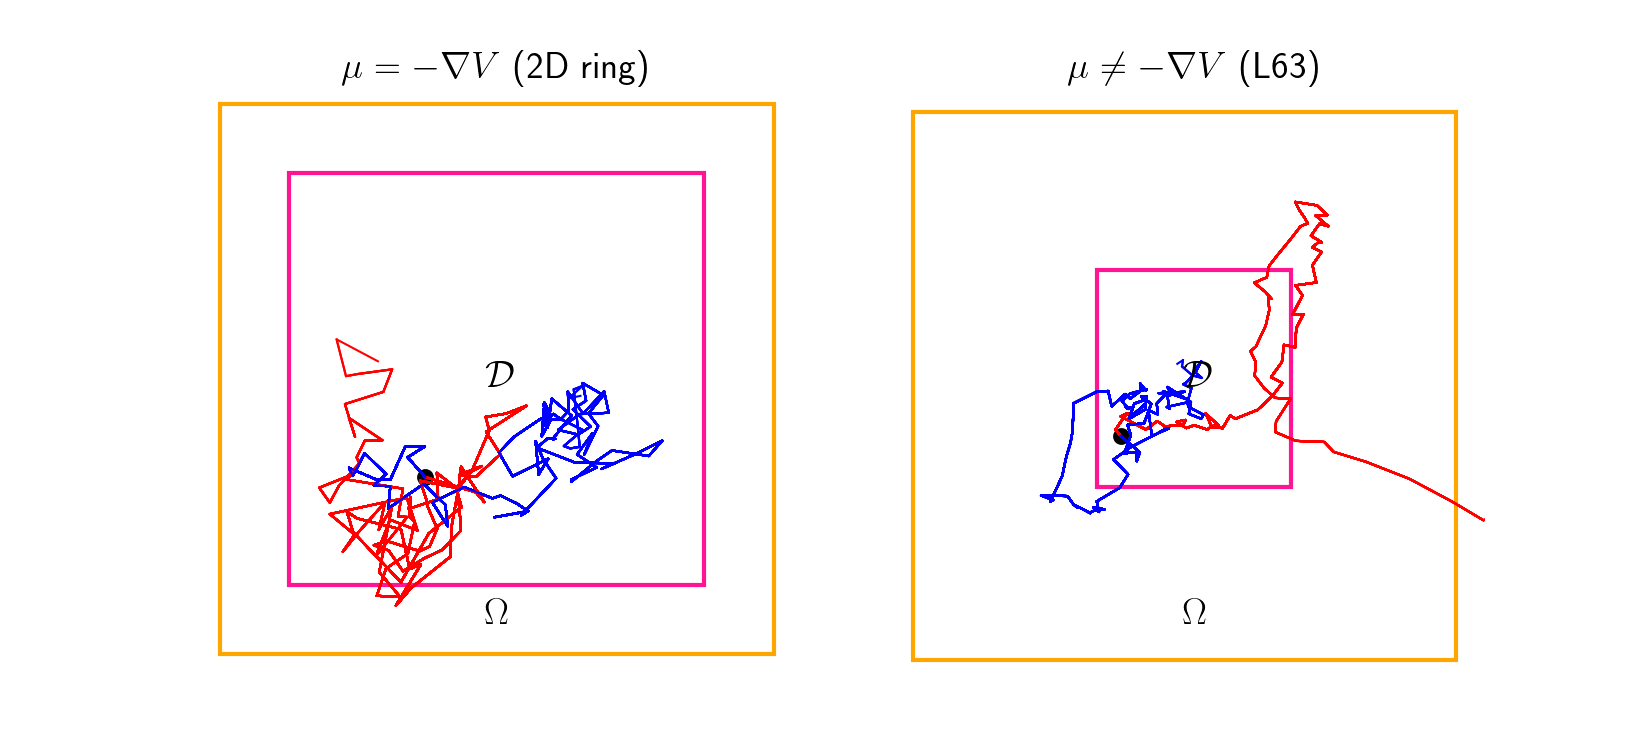
\includegraphics[scale=0.55]{dynamic-fp/plots/dynamic-plots-h-SDE.png}
    \caption{h-SDE trajectories for various systems. In both cases a pair of trajectories start from the same point (depicted as a black dot) in $\mathcal D$. While the trajectories for the gradient system might leave $\mathcal D$ (smaller rectangle), they do not leave $\Omega$ (larger rectangle). However, the same is not true for the non-gradient system.}
    \label{fig:h-SDE--dynamic-fp}
\end{figure}

Our knowledge of $\bar{\mu}$ is determined by our knowledge of $p_\infty$. If we do not have an analytic form for $p_\infty$ and have computed $p_\infty$ (up to the normalization constant) only up to the domain $\Omega$ then we can only be sure of our knowledge of $\bar{\mu}$ up to the domain $\Omega$. Consequently, if we want to compute the solution on the domain $\mathcal D$ then we must select $\mathcal D\subset\Omega$ in a way such that the trajectories of h-SDE that start inside $\mathcal D$, do not leave $\Omega$ till time $T$ with high probability. To quantify this notion, we can choose a tolerance $\varepsilon>0$ and select $\mathcal D, T$ such that,


\begin{align}
    \xi(T, \mathcal D, \Omega)\stackrel{\rm def}{=}\mathbb E_{\mathbf x\sim U(\mathcal D)}[P(\bar X_t\in\Omega\;\forall\;t\in[0, T]|\bar X_0=\mathbf x)] > 1-\varepsilon\label{eq:xi-defn--dynamic-fp}
\end{align}

$\xi(T, \mathcal D, \Omega)$ denotes the average probability that a trajectory stays inside $\Omega$ till time $T$ given that it started inside $\mathcal D$, $U(\mathcal D)$ denotes the uniform distribution on $\mathcal D$ in \eqref{eq:xi-defn--dynamic-fp}. $\xi$ helps us specify the space-time boundaries for the effective employment of algorithm~\ref{algo:hybrid--dynamic-fp}. While for a gradient system, choosing $\Omega$ such that it contains the corresponding attractor, we can make sure that h-SDE trajectories originating from $\mathcal D$ do not leave $\Omega$ with high probability, the same can not be said for a non-gradient system. Figure~\ref{fig:h-SDE--dynamic-fp} shows the difference between h-SDE trajectories for typical gradient and non-gradient systems. Since for gradient systems the h-SDE trajectories do not leave $\Omega$ with high probability, $\xi(T, \mathcal D, \Omega)\approx 1$ for any $T$. In fact, empirically it might evaluate exactly to $1$. But for non-gradient system $\xi(T, \mathcal D, \Omega)$ is a decreasing function of $T$ as seen in figure~\ref{fig:xi--dynamic-fp} and in such cases we select the hyperparameter $T$ for algorithm~\ref{algo:hybrid--dynamic-fp} according to \eqref{eq:xi-defn--dynamic-fp} using a pre-chosen tolerance $\varepsilon$.

\begin{figure}[!ht]
    \centering
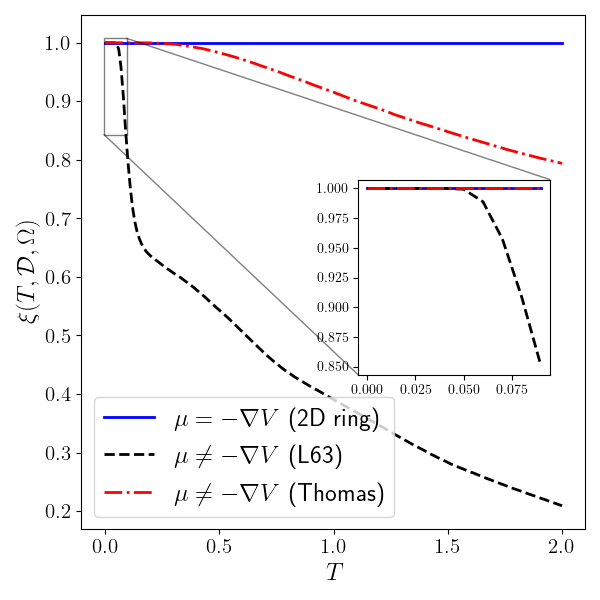
\includegraphics[scale=0.5]{dynamic-fp/plots/dynamic-plots-xi.png}
    \caption{$\xi(T, \mathcal D, \Omega)$ as a function of $T$ for various systems.}
    \label{fig:xi--dynamic-fp}
\end{figure}


We are only able to solve \eqref{eq:FPE-0--dynamic-fp} on a subset $\mathcal D$ of where we solved its stationary counterpart, namely $\Omega$. We refer to this phenomenon as \textit{domain contraction}. Even though we have included gradient systems in the figures~\ref{fig:h-SDE--dynamic-fp}, \ref{fig:xi--dynamic-fp} for expository purposes, since we have perfect knowledge of $p_\infty$ (up to the normalization constant) over entire $\mathbb R^d$, domain contraction is a practical issue only for non-gradient systems and $T$ can be chosen arbitrarily large for gradient systems. 


\subsubsection{Interpretation of finite time viability for non-gradient systems via Feynman-Kac on finite domains}\label{ssec-interpret-FK-finite--dynamic-fp}
Since we are dealing with finite domains, we can also look at the h-SDE through the lens of the Feynman-Kac formula on finite domains. In order to apply the finite domain version of the Feynman-Kac formula one requires perfect knowledge of the solution at the boundary at all times. In our case we need to know $h(t, \mathbf x)$ on $([0, T)\times{\partial\Omega}) \cup (\{0\}\times\bar{\Omega})$. For the ease of discussion let us define the following quantity,
\begin{align}
    h(t, \mathbf x) = \begin{cases}
        &\Psi(T, \mathbf x),\;\forall\;\mathbf x\in \bar{\Omega},\; t=0\\
        & \Psi(T-t, \mathbf x)\;\forall\;(t,\mathbf x)\in[0, T)\times\partial\Omega
    \end{cases}
\end{align}
Assuming we know $\Psi$, the Feynman-Kac formula for $h$ becomes,
\begin{align}
    h(t, \mathbf x) = \mathbb E\left[\left.\Psi(\tau\wedge T, \bar{X}_{\tau\wedge T})\right\vert \bar X_0=\mathbf x\right]\label{eq:h-E-finite--dynamic-fp}
\end{align}
where $\tau$ denotes the first exit-time of $\bar{X}$ for $\Omega$ or,
\begin{align}
    \tau(\mathbf x) \stackrel{\rm def}{=} \inf\{s>0: \bar X_s\not\in\Omega\} 
\end{align}
For derivations of such formulae the interested reader can refer to theorem~4.4.5 in \cite{gobet2016monte} or theorem~4.2 in chapter~7 of \cite{yong1999stochastic} and its preceding section. Since in reality we only know $h(t, \mathbf x)$ at $t=0$ and therefore have no knowledge of $\Psi(T-t, \mathbf x)$ at any point other than $t=0$, we can hope to effectively use \eqref{eq:h-E-finite--dynamic-fp} only if the trajectories of h-SDE do not exit $\Omega$ till time $T$ with high probability. In such a scenario $\tau\wedge T$ becomes equal to $T$ and we are not forced to evaluate $\Psi$ at any point where we have no knowledge of $\Psi$. Using the finite domain version of Feynman-Kac therefore leads us to similar conclusions as in the previous section, namely, algorithm~\ref{algo:hybrid--dynamic-fp} can be used to solve gradient and non-gradient systems up to arbitrarily large and finite times respectively.

\subsubsection{Effect allowing h-SDE trajectories to leave \texorpdfstring{$\Omega$}{Lg} in case of perfect knowledge of \texorpdfstring{$p_\infty$ in $\Omega$}{Lg}}\label{sssec-error--dynamic-fp}
 Since $p_\infty$ is not computed by algorithm~\ref{algo:hybrid--dynamic-fp} but rather is an input to it, a scenario of interest is when we have perfect (rather than approximate) knowledge of $p_\infty$ on $\Omega$. In such a scenario we would like the algorithm to produce reasonably good approximate solutions even when we are willing tolerate $\xi(T, \mathcal D, \Omega)\neq1$ or some h-SDE trajectories leaving $\Omega$ within our chosen $T$. To analyze this scenario let us define our knowledge of $p_\infty$ as,
 \begin{align}
     \hat p_\infty(\mathbf x) =\begin{cases}
         &p_\infty(\mathbf x), \qquad\mathbf x\in\Omega\\
         &p_\infty^\sharp(\mathbf x),\qquad\mathbf x\in\Omega^c
     \end{cases} 
 \end{align}
 where $p_\infty^\sharp\neq p_\infty$ represents imperfect knowledge of $p_\infty$ outside $\Omega$. Similarly we can define a modified h-SDE as,
 \begin{align}
     d\hat X_t = (\sigma^2\nabla\log \hat p_\infty -\mu)\,dt+\sigma\,dW_t
 \end{align} 
 and the corresponding solution generated by algorithm~\ref{algo:hybrid--dynamic-fp} as,
 \begin{align}
   &\hat h(t, \mathbf x) = \mathbb E\left[\left.\frac{p_0(\hat{X}_t)}{\hat{p}_\infty(\hat{X}_t)}\right\vert \hat{X}_0=\mathbf x\right]\\
   & \hat p(t ,\mathbf x)=\hat h(t, \mathbf x) \hat p_\infty(\mathbf x)
\end{align}
Now we are ready to analyze the pointwise error incurred when we allow h-SDE trajectories to escape $\Omega$ within time $T$ with probability less than $\varepsilon$ or $\xi(T, \mathcal D, \Omega)>1-\varepsilon$.
\begin{prop}Let $\bar E, \hat E$ be the events\footnote{Note that $\bar E, \hat E$ are events dependent on $t, \mathbf x$ but to avoid notational cluttering we do not make this dependence explicit.} that $\bar X, \hat X$ stay inside $\Omega$ till time $t$ after starting at $\mathbf x\in\mathcal D\subset\Omega$ respectively. Assume the following,
    \begin{enumerate}
    \item $\xi(T, \mathcal D, \Omega)>1-\varepsilon$
    % \item  \begin{align}\mathbb E_{\mathbf x\sim U(\mathcal D)}[P(\hat E)]\le1-\varepsilon>0\;\forall\;t\in[0, T]\end{align}
    
    \item $\exists$ a constant $K>0$ such that,
    \begin{align} 
     p_\infty(\mathbf x)\,\mathbb E[ h_0(\bar X_t)|\bar X_0=\mathbf x, \bar E^c],\;\hat p_\infty(\mathbf x)\,\mathbb E[\hat h_0(\hat X_t)|\hat X_0=\mathbf x, \hat E^c] < K \;\forall\;\mathbf (t,\mathbf x)\in[0, T]\times\mathcal D
    \end{align}
    where,\begin{align}
    &h_0 \stackrel{\rm def}{=} \frac{p_0}{p_\infty}\\
    &\hat h_0 \stackrel{\rm def}{=} \frac{p_0}{\hat p_\infty}
\end{align}
\end{enumerate}
Then, 
\begin{align}
    \mathbb E_{\mathbf x\sim U(\mathcal D)}[|\hat p(t, \mathbf x)-p(t, \mathbf x)|] \le 2K\varepsilon\;\forall\;t\in[0, T]
    \label{eq:pt-error--dynamic-fp}
\end{align}\label{prop:escape--dynamic-fp}
\end{prop}
\begin{proof}
Let $\mathbf x\in\mathcal D$ and $\Delta_h = h_0-\hat h_0$.
    \begin{align}
    |\hat p(t, \mathbf x)-p(t, \mathbf x)| = |\Delta_1+\Delta_2|    
    \end{align}
where
\begin{align}
    \Delta_1 =  p_\infty(\mathbf x)\,\mathbb E\left[\left.\frac{p_0(\bar{X}_t)}{{p}_\infty(\bar{X}_t)}\right\vert \bar{X}_0=\mathbf x\right]-\hat p_\infty(\mathbf x)\,\mathbb E\left[\left.\frac{p_0(\bar{X}_t)}{\hat{p}_\infty(\bar{X}_t)}\right\vert \bar{X}_0=\mathbf x\right]
\end{align}
and,
\begin{align}
    \Delta_2 = \hat p_\infty(\mathbf x)\,\mathbb E\left[\left.\frac{p_0(\bar{X}_t)}{\hat{p}_\infty(\bar{X}_t)}\right\vert \bar{X}_0=\mathbf x\right]-\hat p_\infty(\mathbf x)\,\mathbb E\left[\left.\frac{p_0(\hat{X}_t)}{\hat{p}_\infty(\hat{X}_t)}\right\vert \hat{X}_0=\mathbf x\right]
\end{align}
Now note that, 
\begin{align}
    \Delta_1 = &p_\infty(\mathbf x)\,\mathbb E[h_0(\bar X_t)|\bar X_0=\mathbf x, \bar E]\,P(\bar E)+p_\infty(\mathbf x)\,\mathbb E[h_0(\bar X_t)|\bar X_0=\mathbf x, \bar E^c]\,(1-P(\bar E))\\
    -&\hat p_\infty(\mathbf x)\,\mathbb E[\hat h_0(\bar X_t)|\bar X_0=\mathbf x, \bar E]\,P(\bar E)-\hat p_\infty(\mathbf x)\,\mathbb E[\hat h_0(\bar X_t)|\bar X_0=\mathbf x, \bar E^c]\,(1-P(\bar E))
\end{align}
Recalling that we have perfect knowledge of $p_\infty$ inside $\Omega$ we get,
\begin{align}
    \Delta_1=&p_\infty(\mathbf x)\left[\mathbb E[\Delta_h(\bar X_t)|\bar X_0=\mathbf x, \bar E]\,P(\bar E)+\mathbb E[\Delta_h(\bar X_t)|\bar X_0=\mathbf x, \bar E^c]\,(1-P(\bar E))\right]\\
    =&p_\infty(\mathbf x)\,\mathbb E[\Delta_h(\bar X_t)|\bar X_0=\mathbf x, \bar E^c]\,(1-P(\bar E))
\end{align}
where we arrive at the last equality by noticing that $\Delta_h=0$ in the event of $\bar E$.
And,
\begin{align}
    \Delta_2 = &\hat p_\infty(\mathbf x)\,[\mathbb E[\hat h_0(\bar X_t)|\bar X_0=\mathbf x, \bar E]\,P(\bar E)+\mathbb E[\hat h_0(\bar X_t)|\bar X_0=\mathbf x, \bar E^c]\,(1-P(\bar E))]\\
    -&\hat p_\infty(\mathbf x)\,[\mathbb E[\hat h_0(\hat X_t)|\hat X_0=\mathbf x, \hat E]\,P(\hat E)+\mathbb E[\hat h_0(\hat X_t)|\hat X_0=\mathbf x, \hat E^c]\,(1-P(\hat E))]
\end{align}
  Since $\bar X, \hat X$ follow identical dynamics inside $\Omega$, $P(\bar E)=P(\hat E)$ and we have,
\begin{align}
    \Delta_2 = &\hat p_\infty(\mathbf x)\,[\mathbb E[\hat h_0(\bar X_t)|\bar X_0=\mathbf x, \bar E^c]-\mathbb E[\hat h_0(\hat X_t)|\hat X_0=\mathbf x, \hat E^c]]\,(1-P(\hat E))
\end{align}
\end{proof}
Again noting $\hat p_\infty(\mathbf x)=p_\infty(\mathbf x)$ and $P(\bar E)=P(\hat E)$ we get,
\begin{align}
    \Delta_1+\Delta_2 = & [p_\infty(\mathbf x)\,\mathbb E[ h_0(\bar X_t)|\bar X_0=\mathbf x, \bar E^c]-\hat p_\infty(\mathbf x)\,\mathbb E[\hat h_0(\hat X_t)|\hat X_0=\mathbf x, \hat E^c]]\,(1-P(\hat E))\\
    \implies|\Delta_1+\Delta_2|\le&2K\,(1-P(\hat E))
\end{align}
Since $\xi$ is a monotone decreasing function of its first argument, the first assumption is equivalent to,
\begin{align}
    \xi(t, \mathcal D, \Omega) > 1-\varepsilon\;\forall\; t\in[0, T]
\end{align}
Therefore, according to the definition of $\xi$,
\begin{align}
    \mathbb E_{\mathbf x\sim U(\mathcal D)}[P(\bar E)] > 1-\varepsilon \;\forall\;t\in[0, T]
\end{align}
which implies,
\begin{align}
    &\mathbb E_{\mathbf x\sim U(\mathcal D)}[1-P(\hat E)] <\varepsilon \;\forall\;t\in[0, T]\\
    \implies&\mathbb E_{\mathbf x\sim U(\mathcal D)}[|\Delta_1+\Delta_2|]<2K\varepsilon
\end{align}
which completes our proof.

The second assumption in proposition~\ref{prop:escape--dynamic-fp} makes sure if we compute the probability densities using only the trajectories that exit $\Omega$ before time $t$, we get bounded quantities independent of $\varepsilon$. Proposition~\ref{prop:escape--dynamic-fp} tells us\textit{, under suitable circumstances, the average error that is caused by allowing some h-SDE trajectories to leave $\Omega$ is proportional to the fraction of trajectories that leave $\Omega$.} If we modify the first assumption to require that the inequality holds pointwise for every $\mathbf x\in\mathcal D$ instead, we can bound the supremum norm of the error over $\mathcal D$ instead of the average error.
\label{ssec-limit--dynamic-fp}